\section{Maximum Likelihood LGM Model Learning}

The starting point of the EM algorithm in the context of model learning relates to the use of Gaussian mixtures to reconstruct an intractable probability density distribution. If Gaussian sums are versatile enough to virtually match any other pdf, relating one outcome of the reconstructed pdf to the mixand it came from is one of the key challenges inherent to Gaussian mixtures. 

In this project, they are utilized to relate a spatial location $L$ with higher and lower-dimensional observations $X$ and $Y$ in a probabilistic manner. This way, a generating model can be constructed to produce missing observations from high-dimensional observations.

The purpose of this phase is to develop the analytic expressions of the Maximum Likelihood Model Learning that will allow us to determine the optimal values of the model's parameters.

For compactness, the full set of parameters appearing in the Gaussian mixture is denoted
\begin{equation}
\Theta =\{\theta^s,\theta^{y,\nu}, \theta^{y,\Sigma}, \theta^{x,\mu}, \theta^{x,\Psi}, \theta^{x,\Lambda}\}\ \mathrm{with}\ s = 1\ ..\ M
\end{equation}
\subsection{}
The complete joint  distribution of the Bayesian Network associated with the plate model reads
\begin{align}
p(s_{1:\bar{N}_R},x_{1:\bar{N}_R},y_{1:\bar{N}_R},\Theta) &= \prod\limits_{i = 1}^{\bar{N}_R}p(s_i = s\vert\theta^s)
p(y_i\vert s_i = s, \theta^{y,\nu}, \theta^{y,\Sigma})p(x_i\vert s_i = s,y_i, \theta^{x,\mu}, \theta^{x,\Psi}, \theta^{x,\Lambda})
\nonumber \\ &=  \prod\limits_{i = 1}^{\bar{N}_R}w_{s_i}\cdot
\mathcal{N}_y\left(\nu_s,\Sigma_s\right)\cdot\mathcal{N}_x\left(\Lambda_sy_i + \mu_s,\Psi_s\right)
\end{align}

By consequent, the Complete Likelihood is
\begin{align}
l_C(\Theta)& = \ln\left(p(s_{1:\bar{N}_R},x_{1:\bar{N}_R},y_{1:\bar{N}_R},\Theta)\right)\nonumber\\
&= \sum\limits_{i = 1}^{\bar{N}_R}\left(\ln(\omega_{s_i}) + \ln\left(\mathcal{N}_y\left(\nu_s,\Sigma_s\right)\right)+ \ln\left(\mathcal{N}_x\left(\Lambda_sy_i + \mu_s,\Psi_s\right)\right)\right) 
\end{align}

But since one does not have access to the index of the mixand responsible for the instanciation of $(x_i,y_i)$, $s_i$ is actually unobservable. The resulting Incomplete Likelihood is given by

\begin{align}
l_I(\Theta)& = \ln\left(p(x_{1:\bar{N}_R},y_{1:\bar{N}_R},\Theta)\right)\nonumber\\
&=  \ln\left(\prod\limits_{i = 1}^{\bar{N}_R}p(x_i,y_i,\Theta)\right)\nonumber\\
&= \ln\left(\prod\limits_{i = 1}^{\bar{N}_R}\sum\limits_{m = 1}^{M}p(s_i = m,x_i,y_i,\Theta)\right)\nonumber\\
&= \ln\left(\prod\limits_{i = 1}^{\bar{N}_R}\sum\limits_{m = 1}^{M}\omega_m\cdot
\mathcal{N}_y\left(y_i\vert\nu_m,\Sigma_m\right)\cdot\mathcal{N}_x\left(x_i\vert\Lambda_my_i + \mu_m,\Psi_m\right)\right)\\
&=\sum\limits_{i = 1}^{\bar{N}_R}\ln\left(\sum\limits_{m = 1}^{M}\omega_m\cdot
\mathcal{N}_y\left(y_i\vert\nu_m,\Sigma_m\right)\cdot\mathcal{N}_x\left(x_i\vert\Lambda_my_i + \mu_m,\Psi_m\right)\right)
\end{align}

Maximum Likelihood pertains to finding the absolute maximum of $l_I$ with respect to the set of parameters $\Theta$. The following presents the analytical derivations ensuring convergence to a local maximum of $l_I$. This procedures is known as the Expectation Maximization Algorithm (EM).
\subsection{}
The EM is an iterative algorithm converging to a local maximum of the likelihood function. It proceeds by successively refining an initial guess of the parameter set $\Theta$. 

\subsubsection{Responsibility}
Let $\gamma(Z_{im})$ be the responsibility of the $m$-th mixand for observations $(x_i,y_i)$. By definition
\begin{equation}
 \gamma(Z_{im})\equiv p(s_i = m\vert x_i,y_i,\Theta)
\end{equation}
From the joint distribution, this becomes
\begin{align}
 \gamma(Z_{im})& = \frac{p(s_i = m, x_i, y_i, \Theta)}{\sum\limits_{m = 1}^{M}p(s_i = m, x_i, y_i, \Theta)}\\
 &=  \frac{w_{m}\cdot
\mathcal{N}_y\left(y_i\vert\nu_m,\Sigma_m\right)\cdot\mathcal{N}_x\left(x_i\vert\Lambda_my_i + \mu_m,\Psi_m\right)}{\sum\limits_{m = 1}^{M}p(s_i = m, x_i, y_i, \Theta)}\\
&=  \frac{w_{m}\cdot
\mathcal{N}_y\left(y_i\vert\nu_m,\Sigma_m\right)\cdot\mathcal{N}_x\left(x_i\vert\Lambda_my_i + \mu_m,\Psi_m\right)}{\sum\limits_{k = 1}^{M}\omega_k\cdot
\mathcal{N}_y\left(y_i\vert\nu_k,\Sigma_k\right)\cdot\mathcal{N}_x\left(x_i\vert\Lambda_ky_i + \mu_k,\Psi_k\right) }
\end{align}

The responsibility acts as a weighing coefficient when updating the parameters of the different mixands. 
\subsubsection{EM parameter updates}
The goal of the EM algorithm is to find a stationary point of the ICLL, $\Theta^*$. To this end, the partial derivatives of the ICLL with respect to the different model parameters need to be computed and set to zero so as to extract the parameter update.

\paragraph{$y$ parameters}
The two parameters related to $y$ are $\nu_m$ and $\Sigma_m$.

\begin{align}
\frac{\partial l(\Theta)   }{\partial  \nu_m } &=\frac{\partial }{\partial \nu_m}\left( \sum\limits_{i = 1}^{\bar{N}_R}\ln\left(\sum\limits_{k = 1}^{M}\omega_k\cdot
\mathcal{N}_y\left(y_i\vert\nu_k,\Sigma_k\right)\cdot\mathcal{N}_x\left(x_i\vert\Lambda_ky_i + \mu_k,\Psi_k\right)\right)\right)\\
&= \sum\limits_{i = 1}^{\bar{N}_R}
\frac{\frac{\partial }{\partial \nu_m}\left(\sum\limits_{k = 1}^{M}\omega_k\cdot
\mathcal{N}_y\left(y_i\vert\nu_k,\Sigma_k\right)\cdot\mathcal{N}_x\left(x_i\vert\Lambda_ky_i + \mu_k,\Psi_k\right)\right)}{\sum\limits_{k = 1}^{M}\omega_k\cdot
\mathcal{N}_y\left(y_i\vert\nu_k,\Sigma_k\right)\cdot\mathcal{N}_x\left(x_i\vert\Lambda_ky_i + \mu_k,\Psi_k\right) }\\
&= \sum\limits_{i = 1}^{\bar{N}_R}
\frac{\frac{\partial }{\partial \nu_m}\left(\omega_m\cdot
\mathcal{N}_y\left(y_i\vert\nu_m,\Sigma_m\right)\cdot\mathcal{N}_x\left(x_i\vert\Lambda_my_i + \mu_m,\Psi_m\right)\right)}{\sum\limits_{k = 1}^{M}\omega_k\cdot
\mathcal{N}_y\left(y_i\vert\nu_k,\Sigma_k\right)\cdot\mathcal{N}_x\left(x_i\vert\Lambda_ky_i + \mu_k,\Psi_k\right) }\\
&= \sum\limits_{i = 1}^{\bar{N}_R}
\frac{\omega_m\cdot
\frac{\partial }{\partial \nu_m}\left(\mathcal{N}_y\left(y_i\vert\nu_m,\Sigma_m\right)\right)\cdot\mathcal{N}_x\left(x_i\vert\Lambda_my_i + \mu_m,\Psi_m\right)}{\sum\limits_{k = 1}^{M}\omega_k\cdot
\mathcal{N}_y\left(y_i\vert\nu_k,\Sigma_k\right)\cdot\mathcal{N}_x\left(x_i\vert\Lambda_ky_i + \mu_k,\Psi_k\right) }
\end{align}
Since
\begin{equation}
\frac{\partial }{\partial \nu_m}\left(\mathcal{N}_y\left(y_i\vert\nu_m,\Sigma_m\right)\right) = \left(y_i - \nu_m\right)^T\Sigma_m^{-1}\mathcal{N}_y\left(y_i\vert\nu_m,\Sigma_m\right)
\end{equation}
We get
\begin{align}
\frac{\partial l(\Theta)   }{\partial  \nu_m } & = \sum\limits_{i = 1}^{\bar{N}_R}
\frac{\left(y_i - \nu_m\right)^T\Sigma_m^{-1}
\omega_m \mathcal{N}_y\left(y_i\vert\nu_m,\Sigma_m\right)\cdot\mathcal{N}_x\left(x_i\vert\Lambda_my_i + \mu_m,\Psi_m\right)}{\sum\limits_{k = 1}^{M}\omega_k\cdot
\mathcal{N}_y\left(y_i\vert\nu_k,\Sigma_k\right)\cdot\mathcal{N}_x\left(x_i\vert\Lambda_ky_i + \mu_k,\Psi_k\right) }\\
&= \sum\limits_{i = 1}^{\bar{N}_R}
\left(y_i - \nu_m\right)^T\Sigma_m^{-1}\gamma\left(Z_{im}\right)
\end{align}
Setting the partial derivative to zero and using the fact that $\Sigma_m$ is non singular, we finally get
\begin{equation}
\boxed{
\nu_m = \frac{ \sum\limits_{i = 1}^{\bar{N}_R}\gamma\left(Z_{im}\right)y_i}{ \sum\limits_{i = 1}^{\bar{N}_R}\gamma\left(Z_{im}\right)}}
\end{equation}

The same process is repeated to find the $\Sigma_m$ update. Since
\begin{align}
\mathcal{N}_y\left(y_i\vert\nu_m,\Sigma_m\right) &= \frac{\vert\Sigma\vert^{-\frac{1}{2}}}{\sqrt{\left(2\pi\right)^d}}e^{-\frac{1}{2}\left(y_i - \nu_m\right)^T\Sigma^{-1}\left(y_i - \nu_m\right)}\\
&= \frac{e^{-\frac{1}{2}\ln\vert\Sigma\vert}}{\sqrt{\left(2\pi\right)^d}}e^{-\frac{1}{2}\left(y_i - \nu_m\right)^T\Sigma^{-1}\left(y_i - \nu_m\right)}
\end{align}
and using the fact that
\begin{equation}
\frac{\partial \ln\vert\Sigma\vert}{\partial \Sigma} = \Sigma^{-T}
\end{equation}
and\footnote{This result can be proved by starting from the partial derivative of $I = AA^{-1}$ with respect to $A_{ij}$ to get $\frac{\partial A^{-1}}{\partial A_{ij}}$, back substitute it into $\frac{\partial }{\partial A_{ij}}\left(\mathbf{x}^TA^{-1}\mathbf{x}\right)$, and showing that this component is equal to $\left[- A^{-T}\mathbf{x}\mathbf{x}^TA^{-T}\right]_{ij}$} 
\begin{equation}
\frac{\partial }{\partial A}\left(\mathbf{x}^TA^{-1}\mathbf{x}\right) = - A^{-T}\mathbf{x}\mathbf{x}^TA^{-T}
\end{equation}


we get
\begin{align}
\frac{\partial\mathcal{N}_y\left(y_i\vert\nu_m,\Sigma_m\right)}{\partial \Sigma_m} &= -\frac{1}{2}\Sigma_m^{-T}\mathcal{N}_y\left(y_i\vert\nu_m,\Sigma_m\right) \nonumber\\
&+ \frac{1}{2}
\Sigma_m^{-T}\left(y_i - \nu_m\right)\left(y_i - \nu_m\right)^T\Sigma_m^{-T}\mathcal{N}_y\left(y_i\vert\nu_m,\Sigma_m\right) 
\end{align}
Since
\begin{equation}
\frac{\partial l(\Theta)}{\partial \Sigma_m} =   \sum\limits_{i = 1}^{\bar{N}_R}
\frac{\omega_m\cdot
\frac{\partial }{\partial \Sigma_m}\left(\mathcal{N}_y\left(y_i\vert\nu_m,\Sigma_m\right)\right)\cdot\mathcal{N}_x\left(x_i\vert\Lambda_my_i + \mu_m,\Psi_m\right)}{\sum\limits_{k = 1}^{M}\omega_k\cdot
\mathcal{N}_y\left(y_i\vert\nu_k,\Sigma_k\right)\cdot\mathcal{N}_x\left(x_i\vert\Lambda_ky_i + \mu_k,\Psi_k\right) }
\end{equation}
We get
\begin{align}
\frac{\partial l(\Theta)}{\partial \Sigma_m} &=  \frac{1}{2} \sum\limits_{i = 1}^{\bar{N}_R}\gamma\left(Z_{im}\right)(-\Sigma_m^{-T}\nonumber\\
&+ 
\Sigma_m^{-T}\left(y_i - \nu_m\right)\left(y_i - \nu_m\right)^T\Sigma_m^{-T} )
\end{align}
Setting this derivative to the zero matrix and using the positive-definiteness of $\Sigma_m$, we get
\begin{equation}
\boxed{
\Sigma_m = \frac{  \sum\limits_{i = 1}^{\bar{N}_R} \gamma(Z_{im})\left(y_i - \nu_m\right)\left(y_i - \nu_m\right)^T }{  \sum\limits_{i = 1}^{\bar{N}_R}\gamma(Z_{im})}}
\end{equation}
\paragraph{$x$ parameters}
The three parameters related to $x$ are $\Lambda_m$, $\mu_m$ and $\Psi_m$. Starting with $\Lambda_m$,

\begin{align}
\frac{\partial l(\Theta)}{\partial \Lambda_m} &= \sum\limits_{i = 1}^{\bar{N}_R}
\frac{\omega_m\cdot
\mathcal{N}_y\left(y_i\vert\nu_m,\Sigma_m\right)\frac{\partial }{\partial \Lambda_m}\left(\mathcal{N}_x\left(x_i\vert\Lambda_my_i + \mu_m,\Psi_m\right)\right)}{\sum\limits_{k = 1}^{M}\omega_k\cdot
\mathcal{N}_y\left(y_i\vert\nu_k,\Sigma_k\right)\cdot\mathcal{N}_x\left(x_i\vert\Lambda_ky_i + \mu_k,\Psi_k\right) }
\end{align}
From 
\begin{equation}
\frac{\partial }{\partial A}\left(\mathbf{y}^T A\mathbf{x}\right) = \mathbf{y}\mathbf{x}^T
\end{equation}
which can be easily proven by expressing the quadratic form in component form, 
it can be shown that 

\begin{equation}
\frac{\partial }{\partial \Lambda_m}\left(\mathcal{N}_x\left(x_i\vert\Lambda_my_i + \mu_m,\Psi_m\right)\right) = - \frac{1}{2}\left(\Psi^{-1} + \Psi^{-T}\right)\left(-x_iy_i^T + \mu_my_i^T + \Lambda_my_iy_i^T\right)\mathcal{N}_x\left(x_i\vert\Lambda_my_i + \mu_m,\Psi_m\right)
\end{equation}

Assuming that $\Psi$ is symmetric, it reduces to
\begin{equation}
\frac{\partial }{\partial \Lambda_m}\left(\mathcal{N}_x\left(x_i\vert\Lambda_my_i + \mu_m,\Psi_m\right)\right) = -\Psi^{-1}\left(-x_iy_i^T + \mu_my_i^T + \Lambda_my_iy_i^T\right)\mathcal{N}_x\left(x_i\vert\Lambda_my_i + \mu_m,\Psi_m\right)
\end{equation}
Setting the corresponding partial derivative of the ICLL to zero finally yields
\begin{equation}
\boxed{
\Lambda_m =\left(
\sum\limits_{i = 1}^{\bar{N}_R}\gamma(Z_{im})\left[x_i - \mu_m\right]y_i^T\right) \left( \sum\limits_{i = 1}^{\bar{N}_R}\gamma(Z_{im})y_iy_i^T\right)^{-1}
}
\end{equation}

Continuing with $\mu_m$, 
\begin{equation}
\frac{\partial\mathcal{N}_x\left(x_i\vert\Lambda_my_i + \mu_m,\Psi_m\right)}{\partial \mu_m} = \left(x_i - \Lambda_my_i - \mu_m\right)\Psi^{-1}\mathcal{N}_x\left(x_i\vert\Lambda_my_i + \mu_m,\Psi_m\right)
\end{equation}
So
\begin{align}
\frac{\partial l(\Theta)}{\partial \mu_m} &= \sum\limits_{i = 1}^{\bar{N}_R}
\frac{\omega_m\cdot
\mathcal{N}_y\left(y_i\vert\nu_m,\Sigma_m\right)\frac{\partial }{\partial \mu_m}\left(\mathcal{N}_x\left(x_i\vert\Lambda_my_i + \mu_m,\Psi_m\right)\right)}{\sum\limits_{k = 1}^{M}\omega_k\cdot
\mathcal{N}_y\left(y_i\vert\nu_k,\Sigma_k\right)\cdot\mathcal{N}_x\left(x_i\vert\Lambda_ky_i + \mu_k,\Psi_k\right) }\\
&= \sum\limits_{i = 1}^{\bar{N}_r}\gamma(Z_{im})\left(x_i - \Lambda_my_i - \mu_m\right)\Psi^{-1}
\end{align}
Setting this partial to zero and leveraging the positive definiteness of $\Psi$ thus gives
\begin{equation}
\boxed{\mu_m = \frac{\sum\limits_{i = 1}^{\bar{N}_r}\gamma(Z_{im})\left(x_i - \Lambda_my_i\right)}{\sum\limits_{i = 1}^{\bar{N}_r}\gamma(Z_{im})} }
\end{equation}

Finally, since
\begin{align}
\frac{\partial\mathcal{N}_x\left(x_i\vert\Lambda_ky_i + \mu_k,\Psi_k\right)}{\partial \Psi_m} &= -\frac{1}{2}\Psi_m^{-T}\mathcal{N}_x\left(x_i\vert\Lambda_ky_i + \mu_k,\Psi_k\right) \nonumber\\
&+ \frac{1}{2}
\Psi_m^{-T}\left(x_i -\Lambda_my_i - \mu_m\right)\left(x_i -\Lambda_my_i - \mu_m\right)^T\Psi_m^{-T}\mathcal{N}_x\left(x_i\vert\Lambda_ky_i + \mu_k,\Psi_k\right)
\end{align}

We can set the partial derivative of the ICLL with respect to $\Psi$ to zero to get
\begin{equation}
\boxed{
\Psi_m = \frac{  \sum\limits_{i = 1}^{\bar{N}_R} \gamma(Z_{im})\left(x_i -\Lambda_my_i - \mu_m\right)\left(x_i -\Lambda_my_i - \mu_m\right)^T }{  \sum\limits_{i = 1}^{\bar{N}_R}\gamma(Z_{im})}}
\end{equation}

And the mixture weights are still given by
\begin{equation}
\boxed{
\omega_m = \frac{\sum\limits_{i = 1}^{\bar{N}_R}\gamma(Z_{im})}{\bar{N}_R}}
\end{equation}

The implementation of the EM algorithm on the training data led to the BIC scores shown on Figure \ref{fig:bic}.
\begin{figure}[tb]
\centering
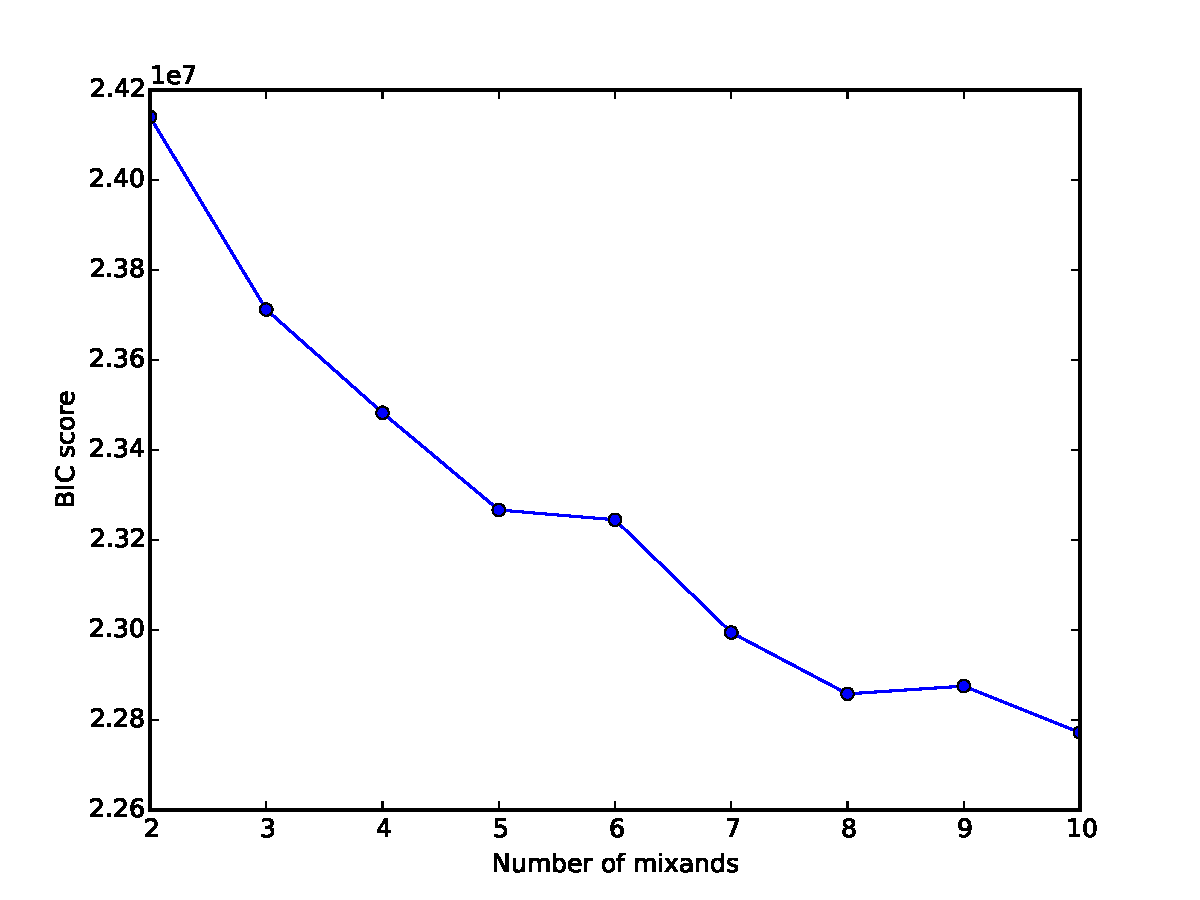
\includegraphics[scale=0.5]{figures_partB/bic}
\caption{BIC score trend against model complexity }
\label{fig:bic}
\end{figure}
Since the BIC score hasn't quite reached a local minimum yet, it seems that more mixands were actually necessary (as pointed out in the Ramos paper, $M=16$ was a better compromise). For the sake of time, we used a model comprised of $M=10$ mixands. 





